% Options for packages loaded elsewhere
% Options for packages loaded elsewhere
\PassOptionsToPackage{unicode}{hyperref}
\PassOptionsToPackage{hyphens}{url}
\PassOptionsToPackage{dvipsnames,svgnames,x11names}{xcolor}
%
\documentclass[
  english,
  11pt,
  a4paper,
  twoside,
  open=any,
  numbers=noenddot]{scrbook}
\usepackage{xcolor}
\usepackage[top=25mm,bottom=28mm,inner=27mm,outer=22mm,headsep=8mm,footskip=12mm]{geometry}
\usepackage{amsmath,amssymb}
\setcounter{secnumdepth}{5}
\usepackage{iftex}
\ifPDFTeX
  \usepackage[T1]{fontenc}
  \usepackage[utf8]{inputenc}
  \usepackage{textcomp} % provide euro and other symbols
\else % if luatex or xetex
  \usepackage{unicode-math} % this also loads fontspec
  \defaultfontfeatures{Scale=MatchLowercase}
  \defaultfontfeatures[\rmfamily]{Ligatures=TeX,Scale=1}
\fi
\usepackage{lmodern}
\ifPDFTeX\else
  % xetex/luatex font selection
\fi
% Use upquote if available, for straight quotes in verbatim environments
\IfFileExists{upquote.sty}{\usepackage{upquote}}{}
\IfFileExists{microtype.sty}{% use microtype if available
  \usepackage[]{microtype}
  \UseMicrotypeSet[protrusion]{basicmath} % disable protrusion for tt fonts
}{}
\makeatletter
\@ifundefined{KOMAClassName}{% if non-KOMA class
  \IfFileExists{parskip.sty}{%
    \usepackage{parskip}
  }{% else
    \setlength{\parindent}{0pt}
    \setlength{\parskip}{6pt plus 2pt minus 1pt}}
}{% if KOMA class
  \KOMAoptions{parskip=half}}
\makeatother
% Make \paragraph and \subparagraph free-standing
\makeatletter
\ifx\paragraph\undefined\else
  \let\oldparagraph\paragraph
  \renewcommand{\paragraph}{
    \@ifstar
      \xxxParagraphStar
      \xxxParagraphNoStar
  }
  \newcommand{\xxxParagraphStar}[1]{\oldparagraph*{#1}\mbox{}}
  \newcommand{\xxxParagraphNoStar}[1]{\oldparagraph{#1}\mbox{}}
\fi
\ifx\subparagraph\undefined\else
  \let\oldsubparagraph\subparagraph
  \renewcommand{\subparagraph}{
    \@ifstar
      \xxxSubParagraphStar
      \xxxSubParagraphNoStar
  }
  \newcommand{\xxxSubParagraphStar}[1]{\oldsubparagraph*{#1}\mbox{}}
  \newcommand{\xxxSubParagraphNoStar}[1]{\oldsubparagraph{#1}\mbox{}}
\fi
\makeatother


\usepackage{longtable,booktabs,array}
\newcounter{none} % for unnumbered tables
\usepackage{calc} % for calculating minipage widths
% Correct order of tables after \paragraph or \subparagraph
\usepackage{etoolbox}
\makeatletter
\patchcmd\longtable{\par}{\if@noskipsec\mbox{}\fi\par}{}{}
\makeatother
% Allow footnotes in longtable head/foot
\IfFileExists{footnotehyper.sty}{\usepackage{footnotehyper}}{\usepackage{footnote}}
\makesavenoteenv{longtable}
\usepackage{graphicx}
\makeatletter
\newsavebox\pandoc@box
\newcommand*\pandocbounded[1]{% scales image to fit in text height/width
  \sbox\pandoc@box{#1}%
  \Gscale@div\@tempa{\textheight}{\dimexpr\ht\pandoc@box+\dp\pandoc@box\relax}%
  \Gscale@div\@tempb{\linewidth}{\wd\pandoc@box}%
  \ifdim\@tempb\p@<\@tempa\p@\let\@tempa\@tempb\fi% select the smaller of both
  \ifdim\@tempa\p@<\p@\scalebox{\@tempa}{\usebox\pandoc@box}%
  \else\usebox{\pandoc@box}%
  \fi%
}
% Set default figure placement to htbp
\def\fps@figure{htbp}
\makeatother


% definitions for citeproc citations
\NewDocumentCommand\citeproctext{}{}
\NewDocumentCommand\citeproc{mm}{%
  \begingroup\def\citeproctext{#2}\cite{#1}\endgroup}
\makeatletter
 % allow citations to break across lines
 \let\@cite@ofmt\@firstofone
 % avoid brackets around text for \cite:
 \def\@biblabel#1{}
 \def\@cite#1#2{{#1\if@tempswa , #2\fi}}
\makeatother
\newlength{\cslhangindent}
\setlength{\cslhangindent}{1.5em}
\newlength{\csllabelwidth}
\setlength{\csllabelwidth}{3em}
\newenvironment{CSLReferences}[2] % #1 hanging-indent, #2 entry-spacing
 {\begin{list}{}{%
  \setlength{\itemindent}{0pt}
  \setlength{\leftmargin}{0pt}
  \setlength{\parsep}{0pt}
  % turn on hanging indent if param 1 is 1
  \ifodd #1
   \setlength{\leftmargin}{\cslhangindent}
   \setlength{\itemindent}{-1\cslhangindent}
  \fi
  % set entry spacing
  \setlength{\itemsep}{#2\baselineskip}}}
 {\end{list}}
\usepackage{calc}
\newcommand{\CSLBlock}[1]{\hfill\break\parbox[t]{\linewidth}{\strut\ignorespaces#1\strut}}
\newcommand{\CSLLeftMargin}[1]{\parbox[t]{\csllabelwidth}{\strut#1\strut}}
\newcommand{\CSLRightInline}[1]{\parbox[t]{\linewidth - \csllabelwidth}{\strut#1\strut}}
\newcommand{\CSLIndent}[1]{\hspace{\cslhangindent}#1}

\ifLuaTeX
\usepackage[bidi=basic,shorthands=off]{babel}
\else
\usepackage[bidi=default,shorthands=off]{babel}
\fi
\ifLuaTeX
  \usepackage{selnolig} % disable illegal ligatures
\fi


\setlength{\emergencystretch}{3em} % prevent overfull lines

\providecommand{\tightlist}{%
  \setlength{\itemsep}{0pt}\setlength{\parskip}{0pt}}



 



% --- ScholarForge common preamble --------------------------------------------
\usepackage{imakeidx}
\makeindex[intoc,columns=2]
\usepackage{microtype}
\setlength{\emergencystretch}{3em}
\widowpenalty=10000
\clubpenalty=10000
\raggedbottom
\providecommand{\sfbookfont}{}

\usepackage[automark]{scrlayer-scrpage}
\clearpairofpagestyles
\ohead{\pagemark}
\ihead{\leftmark}
\setkomafont{pageheadfoot}{\normalfont\small\scshape}
\pagestyle{scrheadings}
\makeatletter
\@ifpackageloaded{tcolorbox}{}{\usepackage[skins,breakable]{tcolorbox}}
\@ifpackageloaded{fontawesome5}{}{\usepackage{fontawesome5}}
\definecolor{quarto-callout-color}{HTML}{909090}
\definecolor{quarto-callout-note-color}{HTML}{0758E5}
\definecolor{quarto-callout-important-color}{HTML}{CC1914}
\definecolor{quarto-callout-warning-color}{HTML}{EB9113}
\definecolor{quarto-callout-tip-color}{HTML}{00A047}
\definecolor{quarto-callout-caution-color}{HTML}{FC5300}
\definecolor{quarto-callout-color-frame}{HTML}{acacac}
\definecolor{quarto-callout-note-color-frame}{HTML}{4582ec}
\definecolor{quarto-callout-important-color-frame}{HTML}{d9534f}
\definecolor{quarto-callout-warning-color-frame}{HTML}{f0ad4e}
\definecolor{quarto-callout-tip-color-frame}{HTML}{02b875}
\definecolor{quarto-callout-caution-color-frame}{HTML}{fd7e14}
\makeatother
\makeatletter
\@ifpackageloaded{bookmark}{}{\usepackage{bookmark}}
\makeatother
\makeatletter
\@ifpackageloaded{caption}{}{\usepackage{caption}}
\AtBeginDocument{%
\ifdefined\contentsname
  \renewcommand*\contentsname{Table of contents}
\else
  \newcommand\contentsname{Table of contents}
\fi
\ifdefined\listfigurename
  \renewcommand*\listfigurename{List of Figures}
\else
  \newcommand\listfigurename{List of Figures}
\fi
\ifdefined\listtablename
  \renewcommand*\listtablename{List of Tables}
\else
  \newcommand\listtablename{List of Tables}
\fi
\ifdefined\figurename
  \renewcommand*\figurename{Figure}
\else
  \newcommand\figurename{Figure}
\fi
\ifdefined\tablename
  \renewcommand*\tablename{Table}
\else
  \newcommand\tablename{Table}
\fi
}
\@ifpackageloaded{float}{}{\usepackage{float}}
\floatstyle{ruled}
\@ifundefined{c@chapter}{\newfloat{codelisting}{h}{lop}}{\newfloat{codelisting}{h}{lop}[chapter]}
\floatname{codelisting}{Listing}
\newcommand*\listoflistings{\listof{codelisting}{List of Listings}}
\usepackage{amsthm}
\theoremstyle{plain}
\newtheorem{theorem}{Theorem}[chapter]
\theoremstyle{plain}
\newtheorem{proposition}{Proposition}[chapter]
\theoremstyle{plain}
\newtheorem{lemma}{Lemma}[chapter]
\theoremstyle{definition}
\newtheorem{definition}{Definition}[chapter]
\theoremstyle{definition}
\newtheorem{exercise}{Exercise}[chapter]
\theoremstyle{definition}
\newtheorem{example}{Example}[chapter]
\theoremstyle{remark}
\AtBeginDocument{\renewcommand*{\proofname}{Proof}}
\newtheorem*{remark}{Remark}
\newtheorem*{solution}{Solution}
\newtheorem{refremark}{Remark}[chapter]
\newtheorem{refsolution}{Solution}[chapter]
\makeatother
\makeatletter
\makeatother
\makeatletter
\@ifpackageloaded{caption}{}{\usepackage{caption}}
\@ifpackageloaded{subcaption}{}{\usepackage{subcaption}}
\makeatother
\usepackage{bookmark}
\IfFileExists{xurl.sty}{\usepackage{xurl}}{} % add URL line breaks if available
\urlstyle{same}
% fallback for those not using the hyperref driver hyperxmp:
\makeatletter
\@ifundefined{xmpquote}{\newcommand{\xmpquote}[1]{#1}}{}
\makeatother
\hypersetup{
  pdftitle={Mathematical Foundations of Deep Learning},
  pdfauthor={ScholarForge project},
  pdflang={en},
  colorlinks=true,
  linkcolor={Maroon},
  filecolor={Maroon},
  citecolor={Blue},
  urlcolor={Blue},
  pdfcreator={LaTeX via pandoc}}


\title{Mathematical Foundations of Deep Learning}
\usepackage{etoolbox}
\makeatletter
\providecommand{\subtitle}[1]{% add subtitle to \maketitle
  \apptocmd{\@title}{\par {\large #1 \par}}{}{}
}
\makeatother
\subtitle{A Compact Rigorous Introduction (ScholarForge test edition)}
\author{ScholarForge project}
\date{2026-11-17}
\begin{document}
\frontmatter
\maketitle

\renewcommand*\contentsname{Table of contents}
{
\setcounter{tocdepth}{1}
\tableofcontents
}

\mainmatter
\bookmarksetup{startatroot}

\chapter*{Preface}\label{preface}
\addcontentsline{toc}{chapter}{Preface}

\markboth{Preface}{Preface}

The calculus, linear algebra, optimisation and automatic differentiation
needed to define, train and analyse feedforward neural networks,
presented with proofs at the level of a first graduate course. Out of
scope: architectures beyond feedforward networks, statistical learning
theory beyond the universal approximation theorem, and implementation
details of specific software frameworks.

This textbook is written for readers at the graduate level.

\begin{tcolorbox}[enhanced jigsaw, arc=.35mm, bottomrule=.15mm, bottomtitle=1mm, breakable, colback=white, colbacktitle=quarto-callout-note-color!10!white, colframe=quarto-callout-note-color-frame, coltitle=black, left=2mm, leftrule=.75mm, opacityback=0, opacitybacktitle=0.6, rightrule=.15mm, title=\textcolor{quarto-callout-note-color}{\faInfo}\hspace{0.5em}{How this book was produced}, titlerule=0mm, toprule=.15mm, toptitle=1mm]

The text was drafted with the assistance of an AI model and assembled,
checked and typeset with ScholarForge 0.1.0. Cited works were verified
against bibliographic registries, and formulas with attached checks were
verified by computer algebra; the appendix \emph{Verification report}
lists what was checked, what was not, and what needs expert review.
Machine checks reduce but do not eliminate the possibility of errors.

\end{tcolorbox}

\section*{Conventions}\label{conventions}
\addcontentsline{toc}{section}{Conventions}

\markright{Conventions}

\begin{itemize}
\tightlist
\item
  Vectors are bold lowercase column vectors, matrices bold uppercase;
  the transpose is written with a superscript top.
\item
  The gradient of a scalar function is a column vector; the Jacobian of
  a map has one row per output.
\item
  log is the natural logarithm; {[}P{]} equals 1 if the statement P
  holds and 0 otherwise.
\end{itemize}

\bookmarksetup{startatroot}

\chapter{Calculus}\label{sec-calculus}

\section{Derivatives and the chain
rule}\label{sec-calculus-derivatives-and-the-chain-rule}

Training a neural network means minimising a scalar loss over many
parameters, and every practical method for that minimisation needs
derivatives. This block fixes the basic notions for functions of one
real variable;
Section~\ref{sec-linear-algebra-vectors-matrices-and-gradients} extends
them to several variables.

\begin{definition}[Derivative]\protect\hypertarget{def-derivative}{}\label{def-derivative}

Let \(I \subseteq \mathbb{R}\) be an open interval and
\(f\colon I \to \mathbb{R}\). The function \(f\) is
\emph{differentiable\index{differentiable}} at \(a \in I\) if the limit
\begin{equation}\protect\phantomsection\label{eq-derivative}{
f'(a) = \lim_{h \to 0} \frac{f(a+h) - f(a)}{h}
}\end{equation} exists; the number \(f'(a)\) is the
\emph{derivative\index{derivative}} of \(f\) at \(a\).

\end{definition}

Equivalently, \(f(a+h) = f(a) + f'(a)\,h + r(h)\) with \(r(h)/h \to 0\)
as \(h \to 0\): near \(a\) the function is approximated by an affine map
whose slope is the derivative. This first-order view is the one that
generalises to many variables and to automatic differentiation.

\begin{theorem}[Chain
rule]\protect\hypertarget{thm-chain-rule}{}\label{thm-chain-rule}

Let \(I, J \subseteq \mathbb{R}\) be open intervals, let
\(g\colon I \to J\) be differentiable at \(a\) and let
\(f\colon J \to \mathbb{R}\) be differentiable at \(g(a)\). Then
\(f \circ g\) is differentiable at \(a\) and
\begin{equation}\protect\phantomsection\label{eq-chain-rule}{
(f\circ g)'(a) = f'\big(g(a)\big)\, g'(a).
}\end{equation}

\end{theorem}

\begin{proof}
Define \(\varphi(y) = \big(f(y) - f(g(a))\big)/\big(y - g(a)\big)\) for
\(y \neq g(a)\) and \(\varphi(g(a)) = f'(g(a))\). Differentiability of
\(f\) at \(g(a)\) means that \(\varphi\) is continuous at \(g(a)\), and
\(f(y) - f(g(a)) = \varphi(y)\,\big(y - g(a)\big)\) holds for every
\(y \in J\). Substituting \(y = g(a+h)\) gives \[
\frac{f(g(a+h)) - f(g(a))}{h} = \varphi\big(g(a+h)\big)\,\frac{g(a+h) - g(a)}{h}.
\] As \(h \to 0\) we have \(g(a+h) \to g(a)\) because \(g\) is
continuous at \(a\), so the first factor tends to \(f'(g(a))\) and the
second to \(g'(a)\).
\end{proof}

The auxiliary function \(\varphi\) avoids dividing by \(g(a+h) - g(a)\),
which can vanish for arbitrarily small \(h \neq 0\); this is the gap in
the tempting argument that simply cancels \(\Delta g\).

\begin{example}[Logistic
sigmoid]\protect\hypertarget{exm-sigmoid-derivative}{}\label{exm-sigmoid-derivative}

The logistic sigmoid\index{logistic sigmoid}
\(\sigma(x) = 1/(1 + e^{-x})\) maps \(\mathbb{R}\) onto \((0,1)\) and is
a classical activation function. Writing \(\sigma = f \circ g\) with
\(g(x) = 1 + e^{-x}\) and \(f(u) = u^{-1}\), the chain rule gives
\(\sigma'(x) = -g(x)^{-2}\cdot(-e^{-x})\), which simplifies to
\begin{equation}\protect\phantomsection\label{eq-sigmoid-derivative}{
\sigma'(x) = \sigma(x)\,\big(1 - \sigma(x)\big).
}\end{equation} Hence \(0 < \sigma'(x) \le \sigma'(0) = 1/4\) for all
\(x\); see Figure~\ref{fig-sigmoid}. Since the bound is attained only at
the origin, a product of many such factors becomes small, which is one
reason why deep networks of sigmoid units are hard to train with
gradient methods (\citeproc{ref-goodfellow2016}{Goodfellow et al.
2017}).

\end{example}

\begin{figure}

\centering{

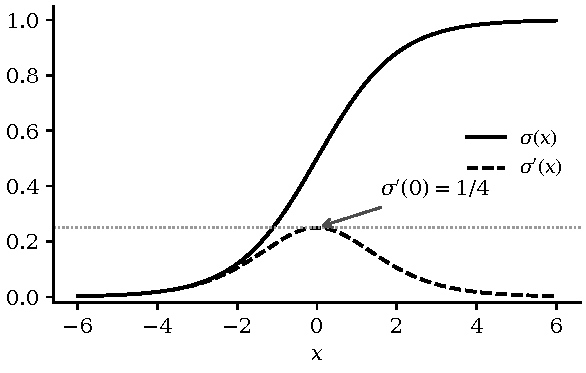
\includegraphics[width=0.8\linewidth,height=\textheight,keepaspectratio,alt={Line plot for x from -6 to 6: an S-shaped solid curve rising from 0 to 1 and passing 0.5 at x = 0, and a bell-shaped dashed curve with maximum 0.25 at x = 0.}]{chapters/../figures/fig-sigmoid.pdf}

}

\caption{\label{fig-sigmoid}The logistic sigmoid \(\sigma\) (solid) and
its derivative \(\sigma'\) (dashed); the derivative never exceeds
\(1/4\).}

\end{figure}%

\begin{exercise}[]\protect\hypertarget{exr-tanh}{}\label{exr-tanh}

Show that \(\tanh(x) = 2\sigma(2x) - 1\) and deduce
\(\tanh'(x) = 1 - \tanh^2(x)\) from Equation~\ref{eq-sigmoid-derivative}
and Theorem~\ref{thm-chain-rule}.

\end{exercise}

\bookmarksetup{startatroot}

\chapter{Linear Algebra}\label{sec-linear-algebra}

\section{Vectors, matrices and
gradients}\label{sec-linear-algebra-vectors-matrices-and-gradients}

We write vectors as bold lowercase letters and treat them as columns,
\(\mathbf{x} = (x_1, \dots, x_n)^\top \in \mathbb{R}^n\); matrices are
bold uppercase, \(\mathbf{A} \in \mathbb{R}^{m \times n}\), with entries
\(A_{ij}\). The transpose turns rows into columns, and the inner
product\index{inner product} is
\(\langle \mathbf{x}, \mathbf{y}\rangle = \mathbf{x}^\top \mathbf{y} = \sum_i x_i y_i\).

\begin{proposition}[Transpose of a
product]\protect\hypertarget{prp-transpose-product}{}\label{prp-transpose-product}

For \(\mathbf{A} \in \mathbb{R}^{m\times n}\) and
\(\mathbf{B} \in \mathbb{R}^{n\times p}\) we have
\((\mathbf{A}\mathbf{B})^\top = \mathbf{B}^\top \mathbf{A}^\top\).

\end{proposition}

\begin{proof}
The \((i,j)\) entry of \((\mathbf{A}\mathbf{B})^\top\) is the \((j,i)\)
entry of \(\mathbf{A}\mathbf{B}\), namely
\(\sum_{k=1}^n A_{jk} B_{ki}\). The \((i,j)\) entry of
\(\mathbf{B}^\top\mathbf{A}^\top\) is \(\sum_{k=1}^n B_{ki} A_{jk}\),
which is the same sum.
\end{proof}

\begin{definition}[Gradient]\protect\hypertarget{def-gradient}{}\label{def-gradient}

Let \(U \subseteq \mathbb{R}^n\) be open and let
\(f\colon U \to \mathbb{R}\) have all first partial derivatives at
\(\mathbf{x}\). The \emph{gradient\index{gradient}} of \(f\) at
\(\mathbf{x}\) is the column vector
\(\nabla f(\mathbf{x}) = \big(\partial f/\partial x_1, \dots, \partial f/\partial x_n\big)^\top\).

\end{definition}

For a differentiable \(f\) the expansion
\(f(\mathbf{x}+\mathbf{h}) = f(\mathbf{x}) + \nabla f(\mathbf{x})^\top \mathbf{h} + o(\lVert \mathbf{h}\rVert)\)
shows that \(-\nabla f(\mathbf{x})\) is the direction of steepest local
decrease, the fact on which gradient descent in
Section~\ref{sec-optimization-gradient-descent-and-convexity} rests.
More generally, the \emph{Jacobian\index{Jacobian}} of
\(F\colon \mathbb{R}^n \to \mathbb{R}^m\) is the \(m\times n\) matrix
\(J_F\) of first partial derivatives, and the multivariate chain rule
reads
\(J_{F\circ G}(\mathbf{x}) = J_F(G(\mathbf{x}))\,J_G(\mathbf{x})\), the
matrix form of Theorem~\ref{thm-chain-rule}.

\begin{proposition}[Gradient of a quadratic
form]\protect\hypertarget{prp-quadratic-gradient}{}\label{prp-quadratic-gradient}

For \(\mathbf{A}\in\mathbb{R}^{n\times n}\) and the quadratic
form\index{quadratic form}
\(q(\mathbf{x}) = \mathbf{x}^\top \mathbf{A}\mathbf{x}\) we have
\(\nabla q(\mathbf{x}) = (\mathbf{A} + \mathbf{A}^\top)\mathbf{x}\); if
\(\mathbf{A}\) is symmetric,
\(\nabla q(\mathbf{x}) = 2\mathbf{A}\mathbf{x}\).

\end{proposition}

\begin{proof}
Write \(q(\mathbf{x}) = \sum_{i,j} A_{ij} x_i x_j\). Differentiating
with respect to \(x_k\) gives
\(\partial q/\partial x_k = \sum_j A_{kj} x_j + \sum_i A_{ik} x_i\),
which is the \(k\)-th entry of
\(\mathbf{A}\mathbf{x} + \mathbf{A}^\top \mathbf{x}\).
\end{proof}

\begin{example}[Least
squares]\protect\hypertarget{exm-least-squares}{}\label{exm-least-squares}

For a data matrix \(\mathbf{X} \in \mathbb{R}^{m\times n}\) and targets
\(\mathbf{y}\in\mathbb{R}^m\), the loss
\(L(\mathbf{w}) = \tfrac12 \lVert \mathbf{X}\mathbf{w} - \mathbf{y}\rVert^2\)
expands to
\(\tfrac12\mathbf{w}^\top\mathbf{X}^\top\mathbf{X}\mathbf{w} - \mathbf{y}^\top\mathbf{X}\mathbf{w} + \tfrac12\lVert\mathbf{y}\rVert^2\).
Since \(\mathbf{X}^\top\mathbf{X}\) is symmetric,
Proposition~\ref{prp-quadratic-gradient} gives
\begin{equation}\protect\phantomsection\label{eq-least-squares-gradient}{
\nabla L(\mathbf{w}) = \mathbf{X}^\top(\mathbf{X}\mathbf{w} - \mathbf{y}).
}\end{equation} Setting the gradient to zero yields the normal equations
\(\mathbf{X}^\top\mathbf{X}\mathbf{w} = \mathbf{X}^\top\mathbf{y}\),
which have a unique solution exactly when \(\mathbf{X}\) has full column
rank.

\end{example}

\begin{exercise}[]\protect\hypertarget{exr-trace-gradient}{}\label{exr-trace-gradient}

For \(f(\mathbf{W}) = \operatorname{tr}(\mathbf{W}^\top \mathbf{A})\)
with \(\mathbf{W},\mathbf{A}\in\mathbb{R}^{m\times n}\), show that
\(\partial f/\partial W_{ij} = A_{ij}\), so that the gradient of \(f\)
with respect to the matrix \(\mathbf{W}\) is \(\mathbf{A}\) itself.

\end{exercise}

\bookmarksetup{startatroot}

\chapter{Optimization}\label{sec-optimization}

\section{Gradient descent and
convexity}\label{sec-optimization-gradient-descent-and-convexity}

\begin{definition}[Convexity and
smoothness]\protect\hypertarget{def-convex}{}\label{def-convex}

A function \(f\colon \mathbb{R}^n\to\mathbb{R}\) is \emph{convex} if
\(f(\theta\mathbf{x} + (1-\theta)\mathbf{y}) \le \theta f(\mathbf{x}) + (1-\theta) f(\mathbf{y})\)
for all \(\mathbf{x},\mathbf{y}\in\mathbb{R}^n\) and \(\theta\in[0,1]\).
A differentiable \(f\) is \emph{\(L\)-smooth} if
\(\lVert\nabla f(\mathbf{x}) - \nabla f(\mathbf{y})\rVert \le L\lVert\mathbf{x}-\mathbf{y}\rVert\)
for all \(\mathbf{x},\mathbf{y}\).

\end{definition}

Gradient descent\index{gradient descent} with step size \(\eta>0\)
starts from \(\mathbf{x}_0\) and iterates
\begin{equation}\protect\phantomsection\label{eq-gd}{
\mathbf{x}_{k+1} = \mathbf{x}_k - \eta\,\nabla f(\mathbf{x}_k).
}\end{equation} Its analysis rests on a single inequality that bounds
how far \(f\) can rise above its linearisation.

\begin{lemma}[Descent
lemma]\protect\hypertarget{lem-descent}{}\label{lem-descent}

If \(f\) is \(L\)-smooth, then
\(f(\mathbf{y}) \le f(\mathbf{x}) + \nabla f(\mathbf{x})^\top(\mathbf{y}-\mathbf{x}) + \tfrac{L}{2}\lVert\mathbf{y}-\mathbf{x}\rVert^2\)
for all \(\mathbf{x},\mathbf{y}\). In particular, one step of
Equation~\ref{eq-gd} with \(\eta = 1/L\) satisfies
\(f(\mathbf{x}_{k+1}) \le f(\mathbf{x}_k) - \tfrac{1}{2L}\lVert\nabla f(\mathbf{x}_k)\rVert^2\).

\end{lemma}

\begin{proof}
Along the segment \(\mathbf{x}+t(\mathbf{y}-\mathbf{x})\),
\(t\in[0,1]\), the fundamental theorem of calculus gives
\(f(\mathbf{y}) - f(\mathbf{x}) - \nabla f(\mathbf{x})^\top(\mathbf{y}-\mathbf{x}) = \int_0^1 \big(\nabla f(\mathbf{x}+t(\mathbf{y}-\mathbf{x})) - \nabla f(\mathbf{x})\big)^\top(\mathbf{y}-\mathbf{x})\,dt\).
By the Cauchy--Schwarz inequality and \(L\)-smoothness the integrand is
at most \(tL\lVert\mathbf{y}-\mathbf{x}\rVert^2\), and
\(\int_0^1 t\,dt = 1/2\). For the second statement substitute
\(\mathbf{y} = \mathbf{x}_k - \nabla f(\mathbf{x}_k)/L\).
\end{proof}

\begin{theorem}[Convergence of gradient
descent]\protect\hypertarget{thm-gd-convex}{}\label{thm-gd-convex}

Let \(f\) be convex and \(L\)-smooth with a minimiser
\(\mathbf{x}^\star\). Gradient descent with \(\eta = 1/L\) satisfies
\begin{equation}\protect\phantomsection\label{eq-gd-rate}{
f(\mathbf{x}_k) - f(\mathbf{x}^\star) \le \frac{L\,\lVert\mathbf{x}_0 - \mathbf{x}^\star\rVert^2}{2k} \qquad (k\ge 1).
}\end{equation}

\end{theorem}

\begin{proof}
\emph{Sketch.} Write \(f^\star = f(\mathbf{x}^\star)\). Combining
Lemma~\ref{lem-descent} (with \(\eta = 1/L\)) and the convexity
inequality
\(f^\star \ge f(\mathbf{x}_k) + \nabla f(\mathbf{x}_k)^\top(\mathbf{x}^\star - \mathbf{x}_k)\),
and expanding \(\lVert\mathbf{x}_{k+1}-\mathbf{x}^\star\rVert^2\) with
\(\mathbf{x}_{k+1} = \mathbf{x}_k - \nabla f(\mathbf{x}_k)/L\), one
obtains
\begin{equation}\protect\phantomsection\label{eq-gd-telescoping}{
f(\mathbf{x}_{k+1}) - f^\star \le \frac{L}{2}\Big(\lVert\mathbf{x}_k-\mathbf{x}^\star\rVert^2 - \lVert\mathbf{x}_{k+1}-\mathbf{x}^\star\rVert^2\Big).
}\end{equation} Summing Equation~\ref{eq-gd-telescoping} from \(0\) to
\(k-1\) telescopes the right-hand side to at most
\(\tfrac{L}{2}\lVert\mathbf{x}_0-\mathbf{x}^\star\rVert^2\). Since
\(f(\mathbf{x}_i)\) is non-increasing by Lemma~\ref{lem-descent}, the
left-hand side is at least \(k\,\big(f(\mathbf{x}_k) - f^\star\big)\),
which gives Equation~\ref{eq-gd-rate}.
\end{proof}

Complete arguments are given in (\citeproc{ref-boyd2004}{Boyd and
Vandenberghe 2004}) and, together with stochastic variants, in
(\citeproc{ref-bottou2018}{Bottou et al. 2018}). The rate is sublinear:
halving the error requires doubling the number of iterations.

\begin{example}[Quadratic
model]\protect\hypertarget{exm-quadratic-gd}{}\label{exm-quadratic-gd}

For \(f(\mathbf{x}) = \tfrac12\mathbf{x}^\top\mathbf{H}\mathbf{x}\) with
\(\mathbf{H} = \operatorname{diag}(1, 10)\) we have \(L = 10\), and
Equation~\ref{eq-gd} acts coordinate-wise as
\(x_{k+1,i} = (1 - \eta h_i)\,x_{k,i}\). With \(\eta = 1/L\) the first
coordinate contracts by the factor \(0.9\) per step while the second is
annihilated after one step; for \(\eta\) close to \(2/L\) the second
coordinate oscillates, and for \(\eta > 2/L\) it diverges.
Figure~\ref{fig-gd-paths} shows the stable regimes. The ratio \(10\)
between the largest and the smallest curvature, the \emph{condition
number\index{condition number}}, governs the speed of convergence.

\end{example}

\begin{figure}

\centering{

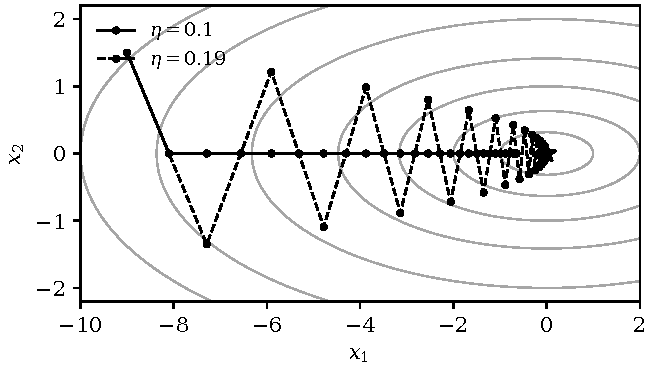
\includegraphics[width=0.85\linewidth,height=\textheight,keepaspectratio,alt={Contour plot of elongated ellipses centred at the origin. The solid path drops straight to the long axis after one step and then creeps along it towards the centre; the dashed path zig-zags across the narrow direction while moving towards the centre.}]{chapters/../figures/fig-gd-paths.pdf}

}

\caption{\label{fig-gd-paths}Gradient descent on
\(f(\mathbf{x}) = \tfrac12(x_1^2 + 10x_2^2)\) from \((-9, 1.5)\) with
\(\eta = 0.1 = 1/L\) (solid) and \(\eta = 0.19\) (dashed), shown over
level sets of \(f\).}

\end{figure}%

In deep learning the loss is neither convex nor globally smooth, and the
gradient is replaced by a stochastic estimate computed on a random
mini-batch of training examples (\citeproc{ref-robbins1951}{Robbins and
Monro 1951}; \citeproc{ref-bottou2018}{Bottou et al. 2018}). The convex
theory nevertheless explains the role of the step size and of curvature.

\begin{exercise}[]\protect\hypertarget{exr-gd-step}{}\label{exr-gd-step}

For \(f(x) = \tfrac{a}{2}x^2\) with \(a>0\), show that gradient descent
converges for every starting point if and only if \(0 < \eta < 2/a\).

\end{exercise}

\bookmarksetup{startatroot}

\chapter{Automatic Differentiation}\label{sec-automatic-differentiation}

\section{Forward and reverse
mode}\label{sec-automatic-differentiation-forward-and-reverse-mode}

A program that computes \(f\colon\mathbb{R}^n\to\mathbb{R}\) from
elementary operations defines a \emph{computational
graph\index{computational graph}}: its nodes are intermediate values
\(v_i\), and its edges record which values each operation reads.
Automatic differentiation\index{automatic differentiation} (AD) applies
Theorem~\ref{thm-chain-rule} to this graph and produces derivatives that
are exact up to floating-point rounding. It differs from finite
differences, which suffer from truncation and cancellation errors, and
from symbolic differentiation, which can produce very large expressions
(\citeproc{ref-baydin2018}{Baydin et al. 2015}).

\begin{example}[Forward and reverse sweeps by
hand]\protect\hypertarget{exm-ad-trace}{}\label{exm-ad-trace}

Consider \(f(x_1, x_2) = x_1 x_2 + \sin x_1\), evaluated by the trace
\begin{equation}\protect\phantomsection\label{eq-ad-trace}{
v_1 = x_1,\quad v_2 = x_2,\quad v_3 = v_1 v_2,\quad v_4 = \sin v_1,\quad v_5 = v_3 + v_4 = f ,
}\end{equation} whose graph is drawn in Figure~\ref{fig-comp-graph}.

\emph{Forward mode\index{forward mode}} propagates tangents
\(\dot v_i = \partial v_i/\partial x_1\) together with the values:
\(\dot v_1 = 1\), \(\dot v_2 = 0\),
\(\dot v_3 = \dot v_1 v_2 + v_1\dot v_2\),
\(\dot v_4 = \cos(v_1)\,\dot v_1\) and
\(\dot v_5 = \dot v_3 + \dot v_4\), so that
\(\dot v_5 = x_2 + \cos x_1 = \partial f/\partial x_1\). One forward
sweep yields one directional derivative, hence the full gradient of a
function of \(n\) inputs needs \(n\) sweeps.

\emph{Reverse mode\index{reverse mode}} first evaluates
Equation~\ref{eq-ad-trace} and stores the values, then propagates
adjoints \(\bar v_i = \partial f/\partial v_i\) backwards from
\(\bar v_5 = 1\):
\begin{equation}\protect\phantomsection\label{eq-ad-adjoints}{
\bar v_3 = \bar v_5,\quad \bar v_4 = \bar v_5,\quad \bar v_1 = \bar v_3\, v_2 + \bar v_4\cos v_1,\quad \bar v_2 = \bar v_3\, v_1 .
}\end{equation} A single reverse sweep therefore returns the whole
gradient
\(\nabla f = (\bar v_1, \bar v_2)^\top = (x_2 + \cos x_1,\; x_1)^\top\).

\end{example}

\begin{figure}

\centering{

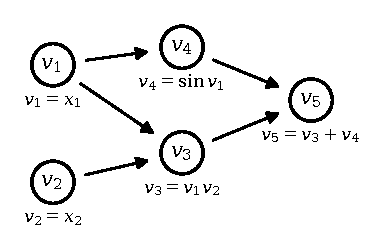
\includegraphics[width=0.75\linewidth,height=\textheight,keepaspectratio,alt={A directed graph with input nodes v1 = x1 and v2 = x2 on the left, a product node v3 and a sine node v4 in the middle, and the output node v5 = v3 + v4 on the right; arrows lead from v1 to v3 and v4, from v2 to v3, and from v3 and v4 to v5.}]{chapters/../figures/fig-comp-graph.pdf}

}

\caption{\label{fig-comp-graph}Computational graph of
\(f(x_1,x_2) = x_1x_2 + \sin x_1\). Forward mode follows the arrows;
reverse mode sends adjoints against them.}

\end{figure}%

\begin{proposition}[Cost of reverse
mode]\protect\hypertarget{prp-reverse-cost}{}\label{prp-reverse-cost}

For a scalar function evaluated by a program with \(N\) elementary
operations, reverse-mode AD computes the full gradient with a number of
operations bounded by a small constant multiple of \(N\), independently
of the number \(n\) of inputs. The price is memory: the intermediate
values of the forward sweep must be stored or recomputed
(\citeproc{ref-griewank2008}{Griewank and Walther 2008}).

\end{proposition}

This \emph{cheap gradient principle} is what makes training networks
with millions of parameters feasible. Backpropagation, derived in
Section~\ref{sec-neural-networks-feedforward-networks-and-backpropagation},
is reverse-mode AD applied to the loss of a network; forward mode
remains preferable when a function has few inputs and many outputs
(\citeproc{ref-baydin2018}{Baydin et al. 2015}).

\begin{exercise}[]\protect\hypertarget{exr-ad-trace}{}\label{exr-ad-trace}

Write the evaluation trace and the reverse sweep for
\(g(x, y) = e^{xy}/(1 + y^2)\), and check the resulting gradient against
direct differentiation.

\end{exercise}

\bookmarksetup{startatroot}

\chapter{Neural Networks}\label{sec-neural-networks}

\section{Feedforward networks and
backpropagation}\label{sec-neural-networks-feedforward-networks-and-backpropagation}

\begin{definition}[Feedforward
network]\protect\hypertarget{def-mlp}{}\label{def-mlp}

A feedforward network\index{feedforward network} with \(L\) layers maps
an input \(\mathbf{a}^{(0)} = \mathbf{x}\in\mathbb{R}^{n_0}\) to an
output \(\mathbf{a}^{(L)}\) through
\begin{equation}\protect\phantomsection\label{eq-mlp}{
\mathbf{z}^{(\ell)} = \mathbf{W}^{(\ell)}\mathbf{a}^{(\ell-1)} + \mathbf{b}^{(\ell)},\qquad \mathbf{a}^{(\ell)} = \phi\big(\mathbf{z}^{(\ell)}\big),\qquad \ell = 1,\dots,L,
}\end{equation} with weight matrices
\(\mathbf{W}^{(\ell)}\in\mathbb{R}^{n_\ell\times n_{\ell-1}}\), bias
vectors \(\mathbf{b}^{(\ell)}\in\mathbb{R}^{n_\ell}\) and an activation
function \(\phi\) applied entrywise; in the output layer \(\phi\) is
often replaced by the identity or by softmax\index{softmax}.

\end{definition}

In this chapter \(L\) counts layers; it is unrelated to the smoothness
constant of
Section~\ref{sec-optimization-gradient-descent-and-convexity}. For
classification into \(K\) classes the last layer produces scores
\(\mathbf{z}\in\mathbb{R}^K\), which are turned into probabilities by
\(\operatorname{softmax}(\mathbf{z})_k = e^{z_k}/\sum_{j} e^{z_j}\) and
scored with the cross-entropy\index{cross-entropy}
\(\ell(\mathbf{z}, y) = -\log\operatorname{softmax}(\mathbf{z})_y\) of
the true class \(y\).

\begin{proposition}[Gradient of the softmax
cross-entropy]\protect\hypertarget{prp-softmax-gradient}{}\label{prp-softmax-gradient}

With \(\mathbf{p} = \operatorname{softmax}(\mathbf{z})\) and
\(\mathbf{e}_y\) the \(y\)-th standard basis vector,
\(\nabla_{\mathbf{z}}\,\ell = \mathbf{p} - \mathbf{e}_y\).

\end{proposition}

\begin{proof}
We have \(\ell = -z_y + \log\sum_j e^{z_j}\). The derivative of the
second term with respect to \(z_k\) is \(e^{z_k}/\sum_j e^{z_j} = p_k\),
and the derivative of \(-z_y\) is \(-1\) if \(k = y\) and \(0\)
otherwise.
\end{proof}

Backpropagation\index{backpropagation} computes all parameter gradients
with one reverse sweep, as guaranteed by
Proposition~\ref{prp-reverse-cost}. Writing
\(\boldsymbol{\delta}^{(\ell)} = \partial\ell/\partial\mathbf{z}^{(\ell)}\),
the chain rule applied to Equation~\ref{eq-mlp} gives
\begin{equation}\protect\phantomsection\label{eq-backprop}{
\boldsymbol{\delta}^{(\ell)} = \Big(\mathbf{W}^{(\ell+1)\top}\boldsymbol{\delta}^{(\ell+1)}\Big)\odot\phi'\big(\mathbf{z}^{(\ell)}\big),\qquad
\frac{\partial\ell}{\partial\mathbf{W}^{(\ell)}} = \boldsymbol{\delta}^{(\ell)}\,\mathbf{a}^{(\ell-1)\top},\qquad
\frac{\partial\ell}{\partial\mathbf{b}^{(\ell)}} = \boldsymbol{\delta}^{(\ell)},
}\end{equation} where \(\odot\) denotes the entrywise product and the
recursion starts from
\(\boldsymbol{\delta}^{(L)} = \mathbf{p} - \mathbf{e}_y\) by
Proposition~\ref{prp-softmax-gradient}. The procedure was popularised
for training multilayer networks by Rumelhart et al.
(\citeproc{ref-rumelhart1986}{1986}), whose experiments showed that
hidden units come to represent important features of the task.

\begin{example}[A two-layer network by
hand]\protect\hypertarget{exm-two-layer}{}\label{exm-two-layer}

Take one input \(x\), one hidden unit with weight \(w_1\) and sigmoid
activation, one linear output with weight \(w_2\), and the squared loss
\(\ell = \tfrac12\big(w_2\,\sigma(w_1 x) - t\big)^2\) for a target
\(t\). Then
\(\partial\ell/\partial w_2 = \big(w_2\sigma(w_1 x) - t\big)\,\sigma(w_1 x)\)
and, using Equation~\ref{eq-sigmoid-derivative},
\(\partial\ell/\partial w_1 = \big(w_2\sigma(w_1x) - t\big)\,w_2\,\sigma(w_1x)\big(1-\sigma(w_1x)\big)\,x\).
These are exactly the two steps of Equation~\ref{eq-backprop} for this
tiny network.

\end{example}

\begin{exercise}[]\protect\hypertarget{exr-backprop-shapes}{}\label{exr-backprop-shapes}

Check that every product in Equation~\ref{eq-backprop} has compatible
dimensions, and rewrite the recursion for the activation
\(\phi = \tanh\).

\end{exercise}

\section{Universal
approximation}\label{sec-neural-networks-universal-approximation}

How expressive are the networks of Definition~\ref{def-mlp}? A classical
answer concerns networks with a single hidden layer.

\begin{theorem}[Universal
approximation]\protect\hypertarget{thm-universal-approximation}{}\label{thm-universal-approximation}

Let \(\phi\colon\mathbb{R}\to\mathbb{R}\) be continuous and sigmoidal,
that is, \(\phi(t)\to 1\) as \(t\to\infty\) and \(\phi(t)\to 0\) as
\(t\to-\infty\). For every continuous \(f\colon[0,1]^n\to\mathbb{R}\)
and every \(\varepsilon>0\) there exist \(N\in\mathbb{N}\), coefficients
\(\alpha_j, b_j\in\mathbb{R}\) and vectors
\(\mathbf{w}_j\in\mathbb{R}^n\) such that
\begin{equation}\protect\phantomsection\label{eq-universal}{
\sup_{\mathbf{x}\in[0,1]^n}\Big|\,f(\mathbf{x}) - \sum_{j=1}^{N}\alpha_j\,\phi\big(\mathbf{w}_j^\top\mathbf{x} + b_j\big)\Big| < \varepsilon .
}\end{equation}

\end{theorem}

This is Cybenko's theorem (\citeproc{ref-cybenko1989}{Cybenko 1989}).
Hornik (\citeproc{ref-hornik1991}{1991}) showed that density also holds
for every bounded and nonconstant activation, with respect to
\(L^p(\mu)\) criteria for finite input measures \(\mu\), so the
essential ingredient is the multilayer architecture rather than the
particular activation. The logistic sigmoid of
Example~\ref{exm-sigmoid-derivative} is sigmoidal in the above sense.

The theorem is an existence statement. It gives no bound on the width
\(N\) needed for a prescribed \(\varepsilon\), it does not say whether
gradient-based training as in Theorem~\ref{thm-gd-convex} finds suitable
weights, and it says nothing about generalisation from finite data.
Quantitative versions require smoothness assumptions on \(f\), and a
satisfactory explanation of why heavily overparameterised networks
trained by stochastic gradient descent generalise well is still an open
research question (\citeproc{ref-lecun2015}{LeCun et al. 2015}).

\begin{example}[Piecewise-linear
bumps]\protect\hypertarget{exm-relu-hat}{}\label{exm-relu-hat}

With the rectified linear unit \(\operatorname{ReLU}(t) = \max(0,t)\),
the combination
\(h(t) = \operatorname{ReLU}(t) - 2\operatorname{ReLU}(t - \tfrac12) + \operatorname{ReLU}(t-1)\)
is a hat function that vanishes outside \([0,1]\) and peaks at
\(h(\tfrac12) = \tfrac12\). Sums of shifted and scaled hats reproduce
piecewise-linear interpolation, which converges uniformly to any
continuous function on an interval as the mesh is refined: a
constructive glimpse of Theorem~\ref{thm-universal-approximation} in one
dimension, with ReLU\index{ReLU} in place of a sigmoidal
function\index{sigmoidal function}.

\end{example}

\begin{exercise}[]\protect\hypertarget{exr-hat}{}\label{exr-hat}

Show that a suitable sum of \(m+1\) hats with nodes \(0, 1/m, \dots, 1\)
interpolates \(f\) at the nodes, and bound the uniform error when \(f\)
is Lipschitz with constant \(K\).

\end{exercise}

\cleardoublepage
\phantomsection
\addcontentsline{toc}{part}{Appendices}
\appendix

\chapter{Glossary}\label{sec-glossary}

\begin{description}
\tightlist
\item[\textbf{automatic differentiation}]
exact-to-rounding evaluation of derivatives by applying the chain rule
to a program's elementary operations (see
Section~\ref{sec-automatic-differentiation-forward-and-reverse-mode})
\item[\textbf{backpropagation}]
reverse-mode automatic differentiation of a network loss, organised
layer by layer (see
Section~\ref{sec-neural-networks-feedforward-networks-and-backpropagation})
\item[\textbf{computational graph}]
the directed graph of intermediate values of a program and the
elementary operations that produce them (see
Section~\ref{sec-automatic-differentiation-forward-and-reverse-mode})
\item[\textbf{condition number}]
the ratio between the largest and the smallest curvature of a quadratic
objective (see
Section~\ref{sec-optimization-gradient-descent-and-convexity})
\item[\textbf{convex function}]
f(theta x + (1-theta) y) \textless= theta f(x) + (1-theta) f(y) for all
x, y and theta in {[}0, 1{]} (see
Section~\ref{sec-optimization-gradient-descent-and-convexity})
\item[\textbf{cross-entropy}]
the loss -log p\_y of the probability assigned to the true class y (see
Section~\ref{sec-neural-networks-feedforward-networks-and-backpropagation})
\item[\textbf{derivative}]
the limit of the difference quotient (f(a+h) - f(a))/h as h tends to 0,
when it exists (see
Section~\ref{sec-calculus-derivatives-and-the-chain-rule})
\item[\textbf{differentiable}]
a function is differentiable at a point if its derivative exists there
(see Section~\ref{sec-calculus-derivatives-and-the-chain-rule})
\item[\textbf{feedforward network}]
a composition of affine maps z = W a + b and entrywise activations a =
phi(z), layer by layer (see
Section~\ref{sec-neural-networks-feedforward-networks-and-backpropagation})
\item[\textbf{forward mode}]
automatic differentiation that propagates tangents alongside the values
from the inputs to the outputs (see
Section~\ref{sec-automatic-differentiation-forward-and-reverse-mode})
\item[\textbf{gradient}]
the column vector of first partial derivatives of a scalar function (see
Section~\ref{sec-linear-algebra-vectors-matrices-and-gradients})
\item[\textbf{gradient descent}]
the iteration x\_\{k+1\} = x\_k - eta grad f(x\_k) with step size eta
\textgreater{} 0 (see
Section~\ref{sec-optimization-gradient-descent-and-convexity})
\item[\textbf{inner product}]
for column vectors x and y, the scalar x\^{}T y = sum\_i x\_i y\_i (see
Section~\ref{sec-linear-algebra-vectors-matrices-and-gradients})
\item[\textbf{Jacobian}]
the m-by-n matrix of first partial derivatives of a map from R\^{}n to
R\^{}m (see
Section~\ref{sec-linear-algebra-vectors-matrices-and-gradients})
\item[\textbf{L-smooth function}]
a differentiable function whose gradient is Lipschitz continuous with
constant L (see
Section~\ref{sec-optimization-gradient-descent-and-convexity})
\item[\textbf{logistic sigmoid}]
the function sigma(x) = 1/(1 + exp(-x)), mapping the real line onto (0,
1) (see Section~\ref{sec-calculus-derivatives-and-the-chain-rule})
\item[\textbf{quadratic form}]
a function q(x) = x\^{}T A x for a square matrix A (see
Section~\ref{sec-linear-algebra-vectors-matrices-and-gradients})
\item[\textbf{ReLU}]
the rectified linear unit t -\textgreater{} max(0, t) (see
Section~\ref{sec-neural-networks-universal-approximation})
\item[\textbf{reverse mode}]
automatic differentiation that propagates adjoints from the output back
to the inputs after a forward evaluation (see
Section~\ref{sec-automatic-differentiation-forward-and-reverse-mode})
\item[\textbf{sigmoidal function}]
a function tending to 1 at plus infinity and to 0 at minus infinity (see
Section~\ref{sec-neural-networks-universal-approximation})
\item[\textbf{softmax}]
the map z -\textgreater{} (e\^{}\{z\_k\} / sum\_j e\^{}\{z\_j\})\_k from
scores to probabilities (see
Section~\ref{sec-neural-networks-feedforward-networks-and-backpropagation})
\item[\textbf{universal approximation}]
the property that one-hidden-layer networks are dense in the continuous
functions on a compact set (see
Section~\ref{sec-neural-networks-universal-approximation})
\end{description}

\chapter{Notation}\label{sec-notation}

{\def\LTcaptype{none} % do not increment counter
\begin{longtable}[]{@{}
  >{\raggedright\arraybackslash}p{(\linewidth - 2\tabcolsep) * \real{0.5000}}
  >{\raggedright\arraybackslash}p{(\linewidth - 2\tabcolsep) * \real{0.5000}}@{}}
\toprule\noalign{}
\begin{minipage}[b]{\linewidth}\raggedright
Symbol
\end{minipage} & \begin{minipage}[b]{\linewidth}\raggedright
Meaning
\end{minipage} \\
\midrule\noalign{}
\endhead
\bottomrule\noalign{}
\endlastfoot
\(f'(a)\) & derivative of f at a \\
\(\sigma\) & logistic sigmoid function \\
\(\mathbf{x}\) & a column vector (bold lowercase) \\
\(\mathbf{A}\) & a matrix (bold uppercase) \\
\(\nabla f\) & gradient of f, a column vector \\
\(J_F\) & Jacobian matrix of the map F \\
\(\eta\) & step size (learning rate) of gradient descent \\
\(L\) & Lipschitz constant of the gradient (smoothness constant) \\
\(\mathbf{x}^\star\) & a minimiser of the objective \\
\(v_i\) & intermediate value number i of an evaluation trace \\
\(\dot v_i\) & tangent (forward-mode derivative) of v\_i \\
\(\bar v_i\) & adjoint of v\_i, the derivative of the output with
respect to v\_i \\
\(L\) & number of layers of a network \\
\(\mathbf{W}^{(\ell)}\) & weight matrix of layer ell \\
\(\boldsymbol{\delta}^{(\ell)}\) & gradient of the loss with respect to
the pre-activations of layer ell \\
\(\odot\) & entrywise (Hadamard) product \\
\(\phi\) & activation function \\
\(\varepsilon\) & approximation tolerance \\
\end{longtable}
}

\chapter{Verification report}\label{sec-verification-report}

This appendix is generated automatically. It states what was verified
and how.

{\def\LTcaptype{none} % do not increment counter
\begin{longtable}[]{@{}
  >{\raggedright\arraybackslash}p{(\linewidth - 4\tabcolsep) * \real{0.3333}}
  >{\raggedleft\arraybackslash}p{(\linewidth - 4\tabcolsep) * \real{0.3333}}
  >{\raggedright\arraybackslash}p{(\linewidth - 4\tabcolsep) * \real{0.3333}}@{}}
\toprule\noalign{}
\begin{minipage}[b]{\linewidth}\raggedright
Claim status
\end{minipage} & \begin{minipage}[b]{\linewidth}\raggedleft
Count
\end{minipage} & \begin{minipage}[b]{\linewidth}\raggedright
Meaning
\end{minipage} \\
\midrule\noalign{}
\endhead
\bottomrule\noalign{}
\endlastfoot
verified & 7 & proved by exact computer algebra or a formal proof \\
supported & 13 & independent evidence agrees (numerical checks, or
quoted evidence found in a verified source) \\
contested & 1 & speculative/open, or a source does not support it \\
unverified & 4 & no independent evidence yet \\
requires expert review & 0 & a check failed or the claim is
high-stakes \\
\end{longtable}
}

Machine-checked formulas: 17 proved symbolically or formally, 3
supported numerically or dimensionally.

{\def\LTcaptype{none} % do not increment counter
\begin{longtable}[]{@{}lr@{}}
\toprule\noalign{}
Source status & Count \\
\midrule\noalign{}
\endhead
\bottomrule\noalign{}
\endlastfoot
verified & 12 \\
rejected & 1 \\
\end{longtable}
}

Only \emph{verified} sources (existence and metadata confirmed in
Crossref, OpenAlex, arXiv or Open Library) can be cited in this book.

A language model's own review of its text is never counted as
independent verification.

\chapter*{References}\label{references}
\addcontentsline{toc}{chapter}{References}

\markboth{References}{References}

\protect\phantomsection\label{refs}
\begin{CSLReferences}{1}{1}
\bibitem[\citeproctext]{ref-baydin2018}
Baydin, Atilim Gunes, Barak A. Pearlmutter, Alexey Andreyevich Radul,
and Jeffrey Mark Siskind. 2015. {``Automatic Differentiation in Machine
Learning: A Survey.''} arXiv:1502.05767. Preprint, arXiv.
\url{https://arxiv.org/abs/1502.05767}.

\bibitem[\citeproctext]{ref-bottou2018}
Bottou, Léon, Frank E. Curtis, and Jorge Nocedal. 2018. {``Optimization
Methods for Large-Scale Machine Learning.''} \emph{SIAM Review} 60 (2):
223--311. \url{https://doi.org/10.1137/16M1080173}.

\bibitem[\citeproctext]{ref-boyd2004}
Boyd, Stephen, and Lieven Vandenberghe. 2004. \emph{Convex
Optimization}. Cambridge University Press.
\url{https://doi.org/10.1017/CBO9780511804441}.

\bibitem[\citeproctext]{ref-cybenko1989}
Cybenko, G. 1989. {``Approximation by Superpositions of a Sigmoidal
Function.''} \emph{Mathematics of Control, Signals, and Systems} 2 (4):
303--14. \url{https://doi.org/10.1007/BF02551274}.

\bibitem[\citeproctext]{ref-goodfellow2016}
Goodfellow, Ian, Yoshua Bengio, Aaron Courville, and Francis Bach. 2017.
\emph{Deep Learning}. MIT Press.
\url{http://openlibrary.org/books/OL26455783M/Deep_Learning}.

\bibitem[\citeproctext]{ref-griewank2008}
Griewank, Andreas, and Andrea Walther. 2008. \emph{Evaluating
Derivatives: Principles and Techniques of Algorithmic Differentiation,
Second Edition}. Society for Industrial and Applied Mathematics.
\url{https://doi.org/10.1137/1.9780898717761}.

\bibitem[\citeproctext]{ref-hornik1991}
Hornik, Kurt. 1991. {``Approximation Capabilities of Multilayer
Feedforward Networks.''} \emph{Neural Networks} 4 (2): 251--57.
\url{https://doi.org/10.1016/0893-6080(91)90009-T}.

\bibitem[\citeproctext]{ref-lecun2015}
LeCun, Yann, Yoshua Bengio, and Geoffrey Hinton. 2015. {``Deep
Learning.''} \emph{Nature} 521 (7553): 436--44.
\url{https://doi.org/10.1038/nature14539}.

\bibitem[\citeproctext]{ref-robbins1951}
Robbins, Herbert, and Sutton Monro. 1951. {``A Stochastic Approximation
Method.''} \emph{The Annals of Mathematical Statistics} 22 (3):
400--407. \url{https://doi.org/10.1214/aoms/1177729586}.

\bibitem[\citeproctext]{ref-rumelhart1986}
Rumelhart, David E., Geoffrey E. Hinton, and Ronald J. Williams. 1986.
{``Learning Representations by Back-Propagating Errors.''} \emph{Nature}
323 (6088): 533--36. \url{https://doi.org/10.1038/323533a0}.

\end{CSLReferences}


\backmatter


\printindex


\end{document}
